\begin{exo}{}

	${ABCD}$ est un rectangle tel que ${AB} = 6$ et ${AD} = 4$.

	On trace un parallélogramme ${EFGH}$ sur ${ABCD}$ tel que ${AG} = {BH} = {CE} = {DF} = x$.



	\begin{center}
		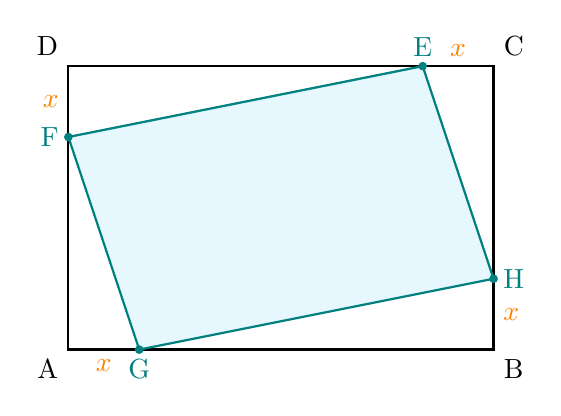
\begin{tikzpicture}[scale=0.9]
			\draw[thick] (0,0) node[below left] {A} -- (6,0) node[below right] {B} -- (6,4) node[above right] {C} -- (0,4) node[above left] {D} -- cycle;
			\coordinate (G) at (1,0);
			\coordinate (H) at (6,1);
			\coordinate (E) at (5,4);
			\coordinate (F) at (0,3);
			\fill[cyan!10] (E) -- (F) -- (G) -- (H) -- cycle;
			\draw[thick, teal] (E) -- (F) -- (G) -- (H) -- cycle;
			\filldraw[teal] (G) circle (1.5pt) node[below] {G};
			\filldraw[teal] (H) circle (1.5pt) node[right] {H};
			\filldraw[teal] (E) circle (1.5pt) node[above] {E};
			\filldraw[teal] (F) circle (1.5pt) node[left] {F};
			\node[orange, below] at (0.5,0) {$x$};
			\node[orange, right] at (6,0.5) {$x$};
			\node[orange, above] at (5.5,4) {$x$};
			\node[orange, left] at (0,3.5) {$x$};
		\end{tikzpicture}
	\end{center}
	\begin{enumerate}
		\item À quel intervalle ${I}$ appartient $x$ ?
		\item Montrer que, pour tout $x \in {I}$, l'aire ${S}(x)$ de ${EFGH}$ est égale à ${S}(x) = 24 - x(6-x) - x(4-x)$ puis que ${S}(x) = 24 - 10x + 2x^2$.
	\end{enumerate}


	On donne la courbe représentative de ${S}$ dans un repère orthogonal :


	\begin{center}
		\begin{tikzpicture}[x=18mm,y=3mm, >=Stealth]
			\def\xmin{0}\def\xmax{4.25}\def\ymin{8}\def\ymax{25.5}
			\draw[gray!40,thin, xstep=0.5, ystep=1] (0,9) grid (\xmax,\ymax);
			\draw[gray!60,thick, xstep=1, ystep=15] (0,9) grid (\xmax,\ymax);
			\draw[thick, ->] (-0.2, 9) -- (\xmax, 9);
			\draw[thick, ->] (0, 7.5) -- (0, \ymax);
			\foreach \x in {1,2,3,4} \draw (\x,9.5) -- (\x,8.5) node[below] {$\x$};
			\foreach \y in {10,15,20} \draw (0.05,\y) -- (-0.05,\y) node[left] {$\y$};
			\draw[domain=0:4, smooth, very thick, orange!70!black] plot (\x, {24 - 10*\x + 2*\x^2});
		\end{tikzpicture}
	\end{center}
	\begin{enumerate}[resume]
		\item Déterminer graphiquement les valeurs de $x$ telles que :
		      \begin{itemize}
			      \item $S(x)$ égale à la moitié de l'aire de $ABCD$
			      \item $S(x)$ égale au deux tiers de l'aire de $ABCD$
			      \item $S(x) = 11,5$
		      \end{itemize}
		      Vérifier ce dernier résultat par un calcul d'image.
		\item En prenant le centimètre pour unité, tracer les différents parallélogrammes $EFGH$ répondant aux points précédents.
		\item À l'aide d'un tableau de valeurs obtenu à la calculatrice, donner une valeur approchée de $x$ au dixième près telle que l'aire de $EFGH$ soit égale aux trois quarts de l'aire de $ABCD$.
	\end{enumerate}
\end{exo}
